\documentclass[
  utf8,%     More capable input encoding than latin-1.
  % parskip,%  For vertical whitespace between paragraphs.  This comes down to more than just using parskip.sty, so it's better to use this class option.
  % S5MP % If you intend to really use margin paragraphs (not recommended!).
%  crop,%     Produce output with crop marks and paper size A4.  Liu-Tryck should like this.  Automatically adds information, including the physical page number, at the top of each page.
       %     Add option 'noInfo' to suppress the info at the top of each page when using option 'crop'.
  % Font options: 'kp' (default), 'times', 'lm'.  The KpFonts (loaded using 'kp'), is the most complete font among the provided options.  Among other, it supports slanted small caps.  See rtthesis.cls for more details regarding the font options.
  largesmallcaps,intlimits,widermath,% Good options to KpFonts.
  sharecounter,nobreak,definition=marks,%  See comments in the results chapter of this document for more information on these options!
  numbers, % If you want to cite references by numbers, use this option.
  noparts% Use option 'noparts' if you do not make use of part divisions.
]{rtthesis}

\usepackage{mythesis}

% !TEX program = pdflatex
% !TEX root = main.tex

\begin{document}
\selectlanguage{english}

\frontmatter
\maketitle

%\begin{abstract}[swedish]
%  Det här som vi har hållit på med är jätteviktigt faktiskt och det vi gjort blev bara sååå bra.  Kanske inte helt otippat, men det glass är sååå gott!

Förresten har vi blivit bäst på att skriva rapporter, så nu ska ska vi inte gå in närmare på några detaljer såhär i sammanfattningen.

%\end{abstract}

\begin{abstract}[english]
  The Equipment Controls and Electronics section (\abbrENSTIECE) at \abbrCERN is developing a high precision piezo-actuated rotational stage for the UA9 crystal collimation project. This collaboration is investigating how tiny bent crystals can help to steer particle beams used in modern hadron colliders such as the Large Hadron Collider (\abbrLHC). Particles are deflected by following the crystal planar channels, "channeling" through the crystal. For high energy particles the angular acceptance for channeling is very low, demanding for a high angular precision mechanism, i.e. the rotational stage. Several control-related issues arising from the complexity and operational environment of the system make it difficult to design a controller that achieves the desired performance. This thesis investigates in different control approaches that could be used to improve the tracking capability of the rotational stage. It shows that the \abbrIRC method could be used to efficiently control the rotational stage. Moreover it shows that a harmonic cancellation method could be used to increase the tracking accuracy by canceling known harmonic disturbances. The harmonic cancellation method (the \abbrRFDC) was implemented in this thesis and proposed as an add-on to the present control algorithm.

\end{abstract}

%\begin{acknowledgments}
  First of all, I would like to thank \abbrCERN and the \abbrENSTIECE section for giving me this opportunity. 

  \addvspace{1em}
  \begin{flushright}
    \textit{%
      Linköping, Augusti 2016\\
      Niklas Ericson%
    }
  \end{flushright}
\end{acknowledgments}


\tableofcontents
\begin{notation}% Passing the option "old" to the notation environment will redefine the notationtabular environment so that it produces an old style LaTeX tabular instead of a ctable.sty style tabular.
  \centering

  % \begin{notationtabular}{Några mängder}{Notation}{Betydelse}
  %   $\naturals$ & Mängden av naturliga tal \\
  %   $\reals$ & Mängden av reella tal \\
  %   $\complexes$ & Mängden av komplexa tal \\
  % \end{notationtabular}

  \begin{notationtabular}{Abbreviations}{Abbreviation}{Meaning}
    \abbrCERN\index{CERN@\abbrCERN!abbreviation} & European Organization for Nuclear Research \\
    \abbrSTM\index{STM@\abbrSTM!abbreviation} & Scanning Tunneling Microscope \\
    \abbrAFM\index{AFM@\abbrAFM!abbreviation} & Atomic Force Microscope \\
    \abbrLHC\index{LHC@\abbrLHC!abbreviation} & Large Hadron Collider \\
    \abbrPEA\index{PEA@\abbrPEA!abbreviation} & Piezoelectric Actuator \\
    \abbrPID\index{PID@\abbrPID!abbreviation} & Proportional, Integral, Derivative (controller) \\
    \abbrDOF\index{DOF@\abbrDOF!abbreviation} & Degrees of Freedom \\
    \abbrPRBS\index{PRBS@\abbrPRBS!abbreviation} & Pseudo Random Binary Sequence \\
    \abbrTF\index{TF@\abbrTF!abbreviation} & Transfer Function \\
    \abbrQFT\index{QFT@\abbrQFT!abbreviation} & Quantitative Feedback Theorem \\
  \end{notationtabular}
\end{notation}


\mainmatter

% !TEX root = main.tex
%en preliminär problemformulering satt i relation till litteraturbasen
\chapter{Introduction}\label{cha:intro}

\section{Background}
High precision positioning systems are vital in e.g. scanning tunneling microscopes (\abbrSTM), atomic force microscopes (\abbrAFM) and in semiconductor lithography. In \abbrAFM, for instance, high precision positioning is required to control the vertical position of the scanning probe to keep the force constant between the sample surface and the probe tip. A topographical image of the sample is obtained by raster-scanning the probe over the sample surface and plotting the vertical displacement against the probe's x-y position. A positioning system that keeps the force constant down to an atomic-scale resolution is thus inevitable in order to obtain a high resolution image without damaging the sample \citep{SurveyOfControlIssues:2007}.

The piezoelectric effect is a phenomenon that arises in certain solid materials when an electric potential is generated in response to applied mechanical stress. The effect was first discovered by Jacques and Pierre Curie in 1880 when they found that applying pressure to a quartz crystal generates electrical potential. Today, the effect is commonly encountered in daily life and utilized in for example lighters, buzzers and loudspeakers.

Smart materials such as piezoelectric and magnetostrictive materials are nowadays commonly used in precision actuators due to their ability to convert electrical energy into mechanical energy. Piezoelectric materials have been commercially available for almost 45 years and have become indispensable for the nanopositioning industry \citep{Piezo:2008}. In cases where a relatively small displacement range is required (travel ranges up to \unit{500}{\micro\meter}) a piezo electric device is the actuator of choice due to its fast response, high resolution and its ability to generate large mechanical forces for small amounts of power in compact designs \citep{SurveyOfControlIssues:2007}.

The \abbrECE (Equipment Controls and Electronics) section in the Engineering Department at \abbrCERN (European Organization for Nuclear Research) is developing a high precision positioning system for use in the UA9 crystal collimation study.

\section{Motivation}
Crystalline solids have the ability to constrain the directions that particles take as they pass through, this is commonly called the "channeling" property. The UA9 collaboration at \abbrCERN is investigating how tiny bent crystals can help to steer particle beams in modern hadron colliders such as the Large Hadron Collider (\abbrLHC) \citep{WebsiteUA9:2016}. In high energy colliders particles tends to drift outwards creating a beam halo. These particles surrounding the beam, can be lost and cause damage to sensitive parts in the accelerator, such as the superconducting magnets which can suffer an abrupt loss in superconducting capability (quench), even from a small dose of deposited energy. To extract and absorb these halo particles, \abbrCERN uses a multi-stage collimation system, consisting of primary and secondary collimators connected in series. \abbrCERN's largest particle accelerator, the \abbrLHC operating at \unit{7}{\tera\electronvolt}, has 108 collimators distributed along 2 beam pipes \citep{CrystalCollimation:2015}. At the moment, these collimators use massive blocks of amorphous material to intercept with the beam and absorb halo particles. The UA9 experiment aims to develop a new collimator, utilizing the technique of a bent crystal and a single absorber which will, in theory, imply in a more efficient cleaning, a less complex system and a reduction of the machine impedance. These are all essential for reaching higher energy levels in a future particle accelerator.

\section{Purpose and goal}
One major difficulty that arises with the use of bent crystals is that, the higher the energy of the particle, the lower the angular acceptance for channeling. Hence, a high precision rotational mechanism is required. For this purpose, the \abbrECE section is developing a rotational stage that will insert and rotate the crystal with a high angular accuracy. The purpose of this thesis is to identify possible control approaches that could be applicable to the rotational stage in order to achieve the desired performance. The stage is required to:
\begin{itemize}
  \item have a total range of \unit{20}{\milli\rad}.
  \item be able to track reference trajectories at ramp rates of \unit{100}{\micro\radianpersecond}.
  \item reject external disturbances to maintain a maximum tracking error of $\pm$\unit{1}{\micro\rad} even when the linear axis is moving.
\end{itemize}

\section{Prospective challenges}\label{sec:prospectiveChallanges}
First of all, piezoelectric actuators show strong nonlinear properties such as hysteresis and creep (drift), which have to be compensated for.\citep{Piezo:2008} Moreover, the mechanical flexural structure in combination with the piezoelectric characteristics leads to a highly resonant structure, making it difficult to achieve the desired performance while operating the rotational stage within noisy environments with external disturbances such as ground vibrations. Furthermore this rotational stage is attached to a linear stage which is composed by a lead-screw, a stepping motor and an axis. The linear movement adds additional perturbation to the rotational stage due to imperfections in the lead-screw and detent torque and stepping nature of the motor. \citep{ButcherController:2015}. Finally, the system changes drastically due to a number of factors such as linear position, linear speed and angular position in combination with a moving center of rotation. The linear dynamic modeling is thereby limited by all these factors requiring a controller that is robust to such variations.

\section{Related work}
During the last couple of decades, a lot of research has been put into the area of nanopositioning and its applications. A well known application is the \abbrAFM discussed in \citep{SurveyOfControlIssues:2007} and \citep{chuang2013robust}, where piezoelectric actuator is commonly used to position the scanning probe tip. The piezoelectric actuator is in many aspects the actuator of choice but its nonlinear characteristics makes it hard to control. A lot of recently published reports discusses the control of piezoelectric actuator \citep{gu2016modeling}, \citep{gu2013motion} and also how to model and compensate for the nonlinear behavior \citep{Maxwell:2012}  \citep{leang2002hysteresis} \citep{ButcherIdentification:2015} \citep{Biggio:2014}.

For the purpose of increasing tracking capability, disturbance rejection and model error robustness in the area of nanopositioning a wide range of controllers have been reported with success. Many of these controller either aims directly to suppress the nonlinear behavior \citep{ompc} \citep{xu2014model} \citep{Elmali:1996} or works in combination with a hysteresis cancellation method \citep{gu:2014} \citep{inputshaper}.

In system suffering from disturbances in a specific frequency region, adding a harmonic cancellation method can efficiently increase the overall tracking performance. Several methods exist where the harmonic cancellation is added either as a feedforward from the modeled disturbance \citep{fujimoto2009rro} \citep{vilanova2008disturbance} or directly in the closed loop \citep{IMP:Perry}.

At \abbrCERN, one attempt to achieve the desired performance has already been made. The proposed controller, presented in \citep{ButcherController:2015} delivers reasonable performance but does not fulfill the requirements during movement. The authors proposes a \abbrPID controller in combination with a prefilter, and a hysteresis compensator. The controller has shown high disturbance rejection at the first resonance peak as well as good tracking performance.

\section{Method}
This thesis aims to identify possible control approaches that can be motivated by simulation and implementation results. The goal can be stated in 2 questions which this thesis aims to provide answers for.

\begin{itemize}
  \item What control approaches can be used to achieve the desired performance?
  \item Which one is the most promising approach with respect to simulated/benchmarked results and ease of implementation on the real device?
\end{itemize}

The methodology that was used to provide answers for these questions is presented in chronological order below.

\begin{itemize}
  \item Literature study.
  \item Further investigation in the selected control approaches.
  \item Benchmarking the selected control approaches in simulations.
  \item Implementation of the most promising approach.
  \item Proposal of a controller.
\end{itemize}

The findings made in the literature study where summarized in a table, see Appendix A, and used to select approaches for further investigation.
All investigated approaches were benchmarked in simulations carried out in Matlab and Simulink, with a linear model of the system. Finally, with performance, stability and implementation considerations, one approach was selected and implemented in LabVIEW to operate on the real device. The final results were used to verify the simulation performance and to give a final evaluation of the controller's applicability and effectiveness.

\section{Limitations}
This thesis have solely focused on control approaches and have thereby excluded all modeling of the system. Extensive modeling had already been carried out on the device, motivating the exclusion. Due to time limitations, only a few control approaches was selected for simulation and only one of them was implemented on the real device. For the same reason, the controller tuning was only carried out until a sufficient set of parameters was found, even though a more optimal set of parameters could have existed at the time.

All simulations will be performed on a linear system model, assuming perfect inverse hysteresis cancellation and a sufficient closed loop to compensate for the creep effect, motivated by the extensive hysteresis model. Furthermore, all controllers will be discretized with a 2kHz sampling frequency for the sake of comparison, even though the number of operations might allow for a higher execution rate.

\section{Outline}
This thesis provides the reader with a detailed description of the system, the theory and simulation results of the selected control methodologies as well as implementation results from benchmark tests with the selected harmonic cancellation approach. The overview presented in Chapter~\ref{cha:systemOverview} provides a brief introduction to collimation and how collimator operates in the \abbrLHC, a more detailed description of the rotational stage including the nonlinear effects that origin from the piezoelectric material. Moreover, a description of the linear identification and the nonlinear compensation is presented in the same chapter as well as an explanation of the present control algorithm. In Chapter~\ref{cha:controlApproach} the simulation results of each controller is presented individually, benchmarked only to the present system. This is followed by two comparison tables gathering comparable results from the stand alone methods and the harmonics cancellation methods , respectively. In Chapter~\ref{cha:exp_result} the experimental results from implementation of the harmonic cancellation is presented and in Chapter~\ref{cha:conclusion} the work is concluded and a final answers to the formulated questions are given.

% !TEX root = main.tex
% en preliminär beskrivning av angreppssätt
\chapter{Method}\label{cha:method}
This thesis will identify possible control approaches that could be applicable to the rotational stage at \abbrCERN in order to meet the performance requirements.
First of all, a brief analysis of the already developed controller will be done in order to point out the drawbacks and determine which controller qualities that have to be improved in order to achieved the desired performance during linear movement of the rotational stage. The main work will then consist of investigating different control approaches such as feedforward, H-infinity, iterative or state feedback control. The most promising approaches will be benchmarked in simulations and compared to the existing algorithm. Finally, the most promising alternative will be implemented and tested on the real rotational stage.

\section{Literature review}
Here follows a review of the preliminary literature base that will be used in this thesis. It will most likely be extended with more articles, papers and books during the work with this thesis.

\subsection*{\citep*{Biggio:2014} {\small \emph{- Memory characteristics of hysteresis and creep in multi-layer piezoelectric actuators: An experimental analysis}}}
The aim of this article is to provide an explanation of peculiar features of the piezoelectric actuator (\abbrPEA) response. It presents an experimental characterization of the nonlinear effects i.e. hysteresis and creep in a \abbrPEA. The authors find that both the instantaneous and delayed response of the PEA have hysteric dependence on the applied voltage level.
Moreover, they present experimental evidence for that the two observed hysteretic relationships share a common memory structure i.e. they are not truly independent nonlinear phenomenas.

\subsection*{\citep*{ButcherIdentification:2015}{\small \emph{- On the identification of Hammerstein systems in the presence of an input hysteretic nonlinearity with nonlocal memory: Piezoelectric actuators – an experimental case study}}}
This paper discusses the identification procedure of the linear dynamic part of piezo based actuators. A Hammerstein structure, consisting of a static (rate independent) hysteresis model with nonlocal memory (the current output does not only depend on the current input voltage but also on its history) and a linear dynamic model, is employed in order to model the hysteretic and dynamic behavior of the actuator.

The authors state that for the identification of the linear part of the actuator, a careful choice of the driving signal has to be made to avoid modifying the characteristics of the excitation. They show that a choice of a \abbrPBRS signal allows the decoupling of the identification of the linear and nonlinear part, since the nonlinear part only transforms the \abbrPBRS signal into another \abbrPBRS.

\subsection*{\citep*{ButcherController:2015} {\small \emph{- Controller Design and Verification for a Rotational Piezo-based Actuator for Accurate Positioning Applications in Noisy Environments}} }
This paper presents the modeling and controller design of a piezo actuated rotational stage operating in a noisy environment at CERN. The authors have adopted a Hammerstein structure, allowing them, in principal, to decouple the nonlinear hysteresis from the linear system dynamics. The extracted linear dynamics is identified as an OE system using several pseudo random binary signals (\abbrPBRS) as excitation signals. By adding different voltage biases to the PBRS it is also verified that the operating voltage point influences the identified transfer function (\abbrTF). The DC gain and the first resonance frequency and amplitude is affected due to the nonlinear piezo properties.

A 2-\abbrDOF controller (feedback and prefilter) and a hysteresis compensator are adopted in order to obtain the desired tracking and disturbance rejection. The proposed controller is designed as a series combination of a \abbrPID controller, a lead network and a 4\textsuperscript{th} order notch filter according to the quantitative feedback theorem (\abbrQFT). The proposed controller is experimentally tested and shows both disturbance rejection and good tracking capability.

\subsection*{\citep*{SurveyOfControlIssues:2007} {\small \emph{- A survey of control issues in nanopositioning}} }
This paper reviews the control-related research in nanopositioning, covering nanopositioning applications, actuators and sensors as well as control challenges. It focuses on piezoelectric actuators discussing both issues in control and different control techniques. Modeling techniques for the nonlinear effects i.e. creep and hysteresis as well as issues such as vibrations and modeling errors are presented in this work. Finally, different control schemes to mitigate the impact from these issues are reviewed such as feedback, forward, iterative and sensor less control.


\subsection*{\citep*{Piezo:2008} {\small \emph{- Piezoelectrics in Positioning, Tutorial on Piezotechnology in Nanopositioning Applications}} }
This tutorial by Physik Instrumente (PI) gives the reader an overview of the fundamentals of piezoelectricity, piezomechanics and piezo actuators as well as detailed information regarding control approaches, environmental dependencies and design of piezoelectric positioning drives/systems. The electrical, mechanical and thermal behavior of piezoelectric actuators is described by basic equations presented in this paper. Several methods to improve the piezo dynamics are also discussed, such as linearization, signal preshaping and InputShaping® which is a patented real-time feedforward technology.

\subsection*{\citep*{FlemingLeang:2014} {\small \emph{- Design, Modeling and Control of Nanopositioning Systems}} }
This book covers the complete design cycle of nanopositioning systems. Some relevant chapters with respect to this thesis are Hysteresis Modeling and Control, Noise in Nanopositioning and Mechanical Design: Flexure-Based Nanopositioners.


\section{Timeplan}
%en tidplan för examensarbetets genomförande inklusive planerade datum för halvtidskontroll och framläggning
Figure~\ref{fig:timeplan} shows the timeplan for the master thesis project. \emph{HP} and \emph{FP} stands for halftime presentation and fulltime presentation, respectively. In addition to the master thesis work, some hardware testing will be carried out from time to time, throughout the whole thesis period.

\begin{figure}[h] %tbp
 \centering %crop: left bottom right top
 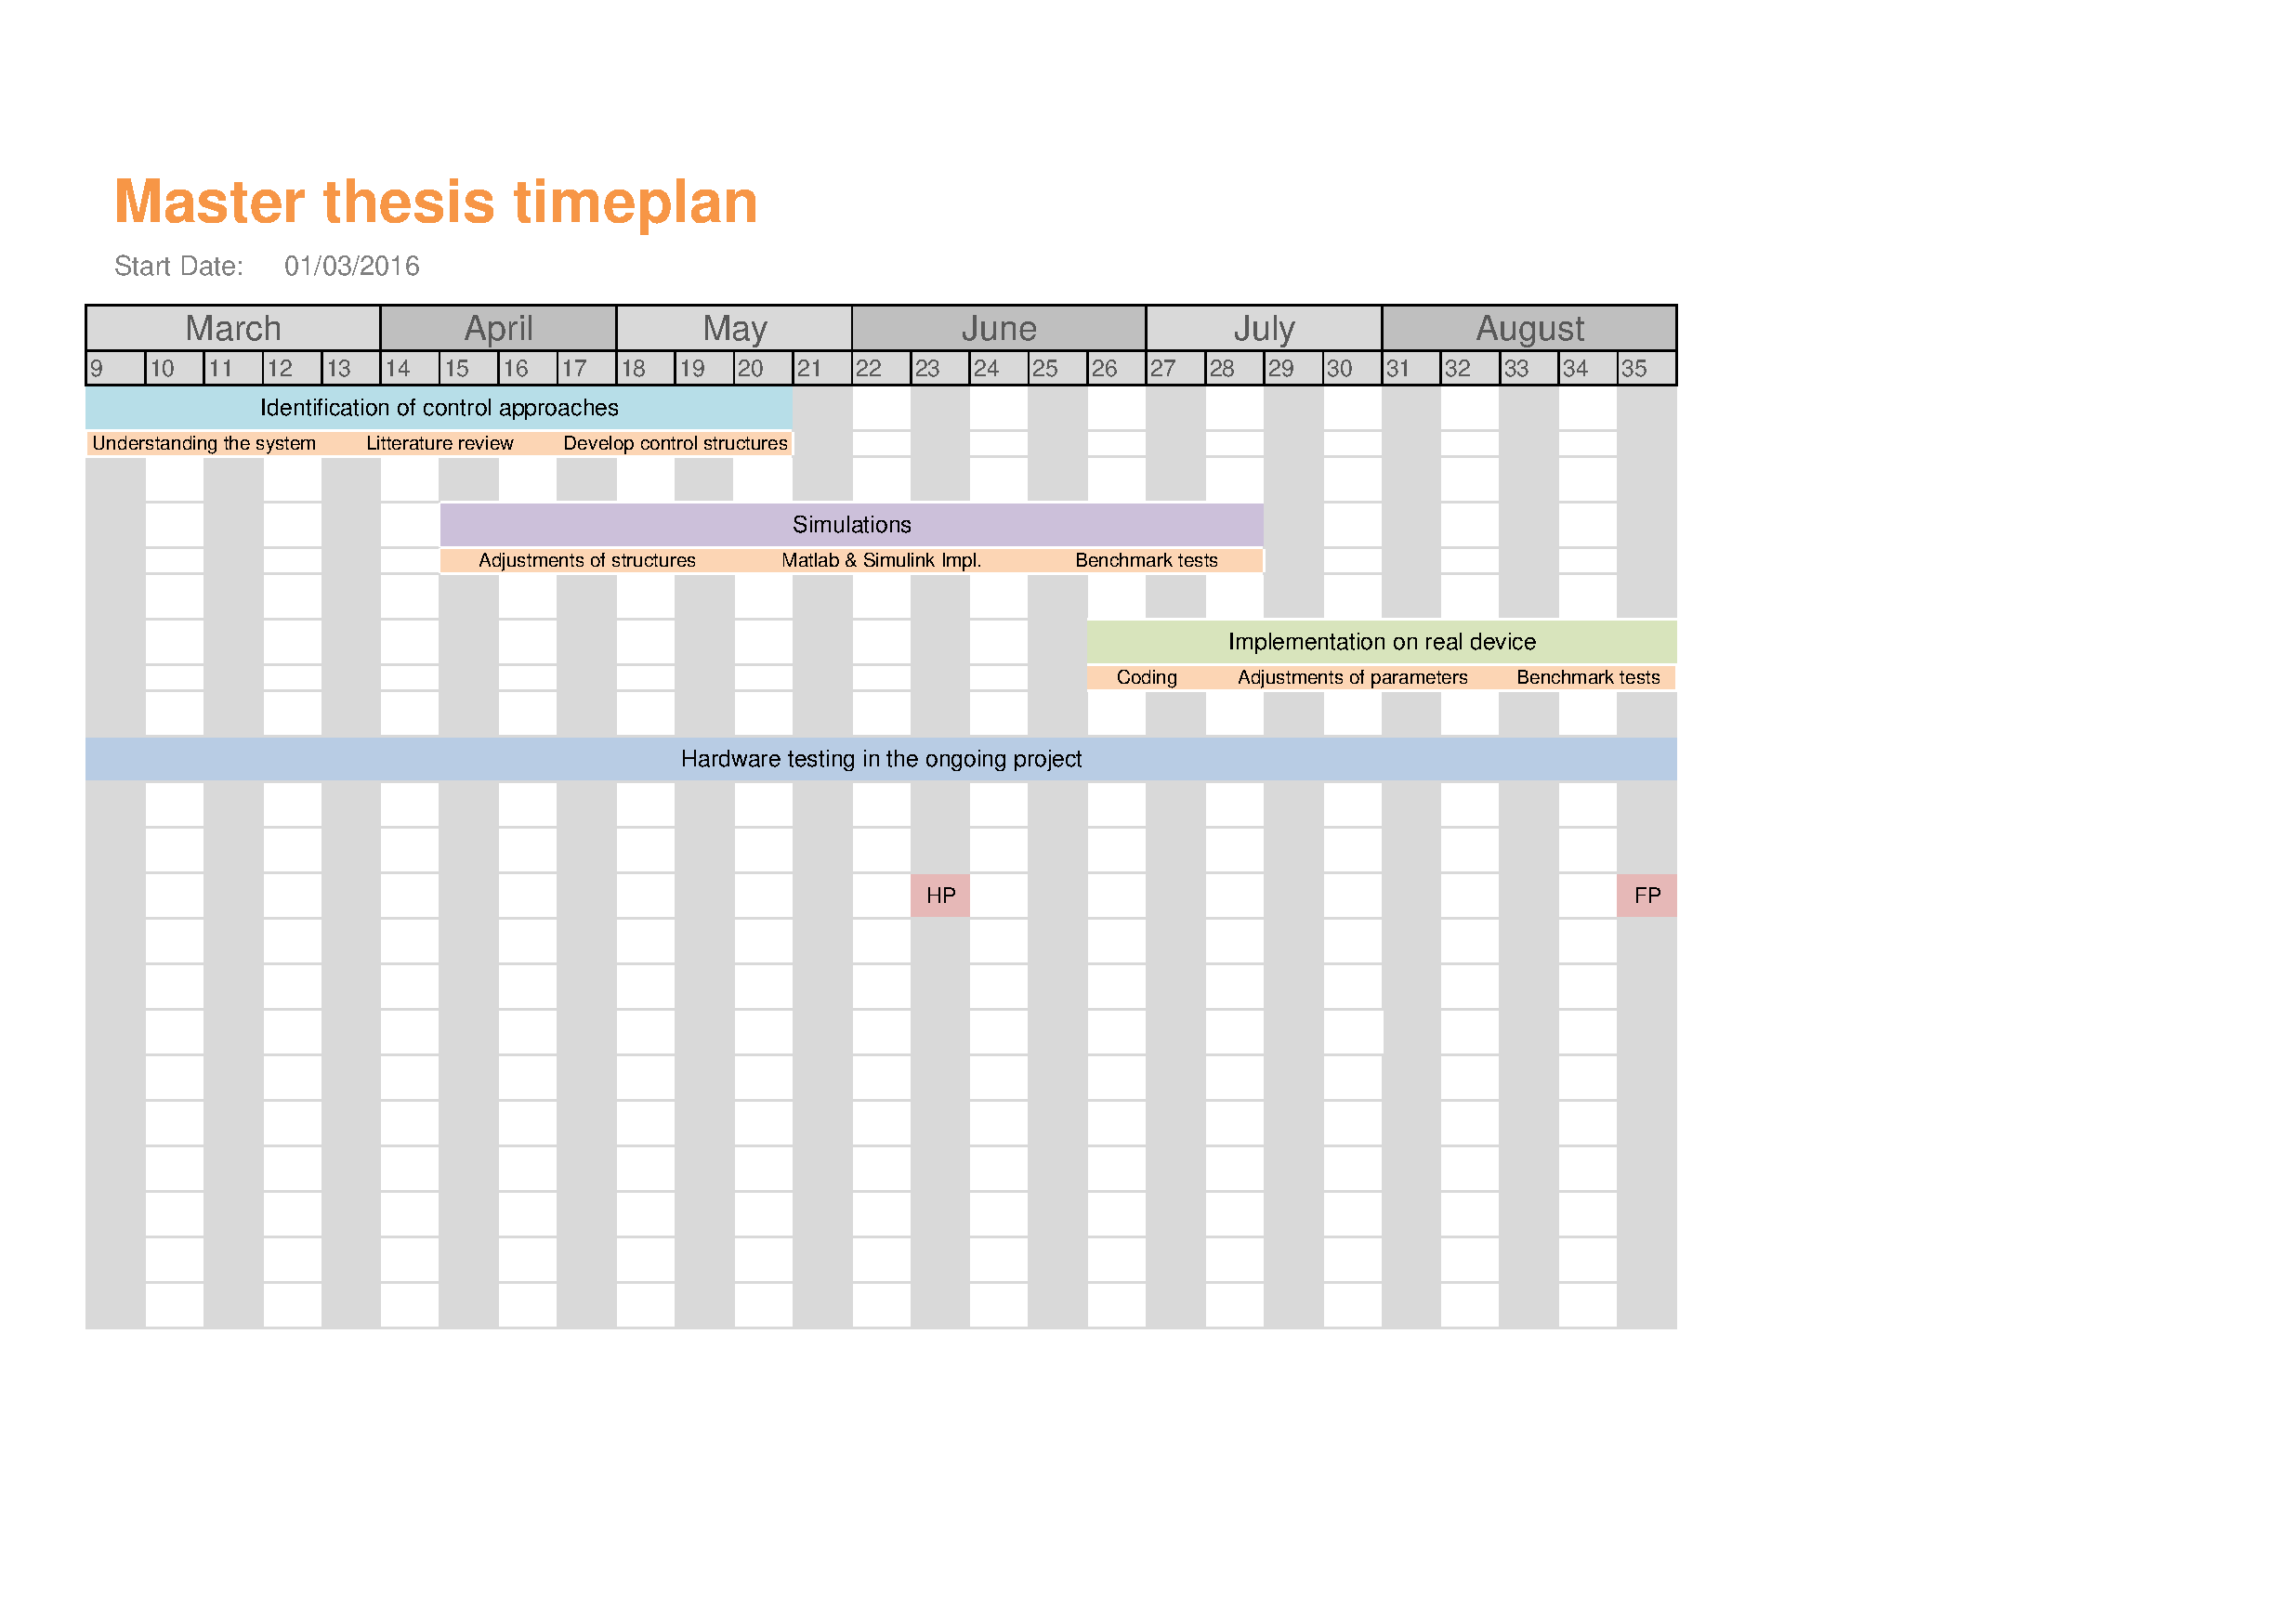
\includegraphics[trim=1cm 12cm 5cm 5.5cm, clip=true, scale=0.42]{fig/timeplan}
 \caption{\label{fig:timeplan}%
 Master Thesis timeplan}
 \end{figure}

\include{report/3_result}
%Sätt av ett kort kapitel sist i rapporten till att avrunda och föreslå rikningar för framtida utveckling av arbetet.
% !TEX root = main.tex
\chapter{Conclusion}\label{cha:conclusion}

This thesis aims to identify, simulate and implement a suitable control approach for a piezo actuated rotational stage at \abbrCERN. The rotational stage is to be used within the UA9 project to position a tiny bent crystal (which will steer particle beams) with a high accuracy. Several control approaches will be simulated in order to find a controller that meet the requirements.



% THESIS PLAN
% % !TEX root = main.tex
%en preliminär problemformulering satt i relation till litteraturbasen
\chapter{Introduction}\label{cha:intro}

\section{Background}
The piezoelectric effect is a phenomenon that arises in certain solid materials when an electric potential is generated in response to applied mechanical stress. The effect was first discovered by Jacques and Pierre Curie in 1880 when they found that applying pressure to a quarz crystal generates electrical potential. Today, the effect is commonly encountered in daily life and utilized in for example lighters, buzzers and loudspeakers.

Smart materials such as piezoelectric and magnetostrictive materials are nowadays commonly used in precision actuators due to their ability to convert electrical energy into mechanical energy. Piezoelectric materials have been commercially available for almost 45 years and have become indispensable for the nanopositioning industry \citep{Piezo:2008}. In cases where a relatively small displacement range is required (travel ranges up to \unit{500}{\micro\meter}) a piezo electric device is the actuator of choice due to its fast response, high resolution and its ability to generate large mechanical forces for small amounts of power in compact designs \citep{SurveyOfControlIssues:2007}.

High precision positioning systems are vital in e.g. scanning tunneling microscopes (\abbrSTM), atomic force microscopes (\abbrAFM) and in semiconductor lithography. In \abbrAFM, for instance, high precision positioning is required to control the vertical position of the scanning probe to keep the force constant between the sample surface and the probe tip. An topographical image of the sample is obtained by raster-scanning the probe over the sample surface and plotting the vertical displacement against the probe's x-y position. A positioning system that keeps the force constant down to an atomic-scale resolution is thus inevitable in order to obtain a high resolution image without damaging the sample \citep{SurveyOfControlIssues:2007}.

The Equipment Controls and Electronics section in the Engineering Department at \abbrCERN (European Organization for Nuclear Research) is developing a high precision positioning system for the control of a piezo-actuated rotational stage used in the UA9 Crystal Collimation study. The stage uses a piezo electric linear stack actuator to displace a flexible lever arm mechanism which generates the rotational movement.

\section{Purpose and Goal}
Crystalline solids have the ability to constrain the directions that particles take as they pass through, this is commonly called the "channelling" property. The UA9 collaboration at \abbrCERN is investigating how tiny bent crystals can help to steer particle beams in modern hadron colliders such as the Large Hadron Collider (\abbrLHC) \citep{WebsiteUA9:2016}. In high energy colliders, such as the \abbrLHC, particles tends to drift outwards creating a beam halo. These particles surrounding the beam, can be lost and cause damage to sensitive parts in the accelerator. By using bent crystals, halo particles can be efficiently extracted from the beam and collected by absorbers further away, reducing the complexity of the system. One major difficulty that aries is that the higher the energy of the particle, the lower the angular acceptance for channeling. Hence, a high precision positioning mechanism with a high angular accuracy is required. The rotational stage (with a range of \unit{20}{\milli\rad}) is of necessity to be able to track reference trajectories at ramp rates of \unit{100}{\micro\radianpersecond} and reject external disturbances to maintain a maximum tracking error of $\pm$\unit{1}{\micro\rad}.

This project aims to identify the possible control approaches that could be applicable to this problem to achieve the desired performance.

\section{Prospective challenges}
First of all, piezoelectric  actuators show strong nonlinear properties such as hysteresis and creep (drift), which have to be compensated for. Moreover, the mechanical flexural structure in combination with the piezo electric characteristics leads to a highly resonant structure, making it difficult to achieve the desired performance while operating the rotational stage within noisy environments with external disturbances such as ground vibrations.

Furthermore this rotational stage is attached to a linear stage which is composed by a leadscrew, a stepping motor and an axel. The linear movement adds additional perturbation to the rotational stage due to imperfections in the leadscrew and detent torque and stepping nature of the motor.

Finally the system dynamics also show linear position dependence requiring a controller that is robust to such variations.

\section{Related work}
One attempt to achieve the desired performance has already been made. The proposed controller, presented in \citep{ButcherController:2015} delivers reasonable performance but does not fulfill the requirements during movement. The authors proposes a PID controller in combination with a pre-filter, and a hysteresis compensator. The controller has shown high disturbance rejection at the first resonance peak as well as good tracking performance.

\section{Outline}
This thesis plan presents an overview of the thesis, including method, literature base and expected results. The method and work flow of the thesis as well as a comprehensive literature review is given in Chapter~\ref{cha:method}. In Chapter~\ref{cha:result} the results that can be expected half way through the project is discussed while a brief summary of the thesis can be found in Chapter~\ref{cha:conclusion}.

% % !TEX root = main.tex
% en preliminär beskrivning av angreppssätt
\chapter{Method}\label{cha:method}
This thesis will identify possible control approaches that could be applicable to the rotational stage at \abbrCERN in order to meet the performance requirements.
First of all, a brief analysis of the already developed controller will be done in order to point out the drawbacks and determine which controller qualities that have to be improved in order to achieved the desired performance during linear movement of the rotational stage. The main work will then consist of investigating different control approaches such as feedforward, H-infinity, iterative or state feedback control. The most promising approaches will be benchmarked in simulations and compared to the existing algorithm. Finally, the most promising alternative will be implemented and tested on the real rotational stage.

\section{Literature review}
Here follows a review of the preliminary literature base that will be used in this thesis. It will most likely be extended with more articles, papers and books during the work with this thesis.

\subsection*{\citep*{Biggio:2014} {\small \emph{- Memory characteristics of hysteresis and creep in multi-layer piezoelectric actuators: An experimental analysis}}}
The aim of this article is to provide an explanation of peculiar features of the piezoelectric actuator (\abbrPEA) response. It presents an experimental characterization of the nonlinear effects i.e. hysteresis and creep in a \abbrPEA. The authors find that both the instantaneous and delayed response of the PEA have hysteric dependence on the applied voltage level.
Moreover, they present experimental evidence for that the two observed hysteretic relationships share a common memory structure i.e. they are not truly independent nonlinear phenomenas.

\subsection*{\citep*{ButcherIdentification:2015}{\small \emph{- On the identification of Hammerstein systems in the presence of an input hysteretic nonlinearity with nonlocal memory: Piezoelectric actuators – an experimental case study}}}
This paper discusses the identification procedure of the linear dynamic part of piezo based actuators. A Hammerstein structure, consisting of a static (rate independent) hysteresis model with nonlocal memory (the current output does not only depend on the current input voltage but also on its history) and a linear dynamic model, is employed in order to model the hysteretic and dynamic behavior of the actuator.

The authors state that for the identification of the linear part of the actuator, a careful choice of the driving signal has to be made to avoid modifying the characteristics of the excitation. They show that a choice of a \abbrPBRS signal allows the decoupling of the identification of the linear and nonlinear part, since the nonlinear part only transforms the \abbrPBRS signal into another \abbrPBRS.

\subsection*{\citep*{ButcherController:2015} {\small \emph{- Controller Design and Verification for a Rotational Piezo-based Actuator for Accurate Positioning Applications in Noisy Environments}} }
This paper presents the modeling and controller design of a piezo actuated rotational stage operating in a noisy environment at CERN. The authors have adopted a Hammerstein structure, allowing them, in principal, to decouple the nonlinear hysteresis from the linear system dynamics. The extracted linear dynamics is identified as an OE system using several pseudo random binary signals (\abbrPBRS) as excitation signals. By adding different voltage biases to the PBRS it is also verified that the operating voltage point influences the identified transfer function (\abbrTF). The DC gain and the first resonance frequency and amplitude is affected due to the nonlinear piezo properties.

A 2-\abbrDOF controller (feedback and prefilter) and a hysteresis compensator are adopted in order to obtain the desired tracking and disturbance rejection. The proposed controller is designed as a series combination of a \abbrPID controller, a lead network and a 4\textsuperscript{th} order notch filter according to the quantitative feedback theorem (\abbrQFT). The proposed controller is experimentally tested and shows both disturbance rejection and good tracking capability.

\subsection*{\citep*{SurveyOfControlIssues:2007} {\small \emph{- A survey of control issues in nanopositioning}} }
This paper reviews the control-related research in nanopositioning, covering nanopositioning applications, actuators and sensors as well as control challenges. It focuses on piezoelectric actuators discussing both issues in control and different control techniques. Modeling techniques for the nonlinear effects i.e. creep and hysteresis as well as issues such as vibrations and modeling errors are presented in this work. Finally, different control schemes to mitigate the impact from these issues are reviewed such as feedback, forward, iterative and sensor less control.


\subsection*{\citep*{Piezo:2008} {\small \emph{- Piezoelectrics in Positioning, Tutorial on Piezotechnology in Nanopositioning Applications}} }
This tutorial by Physik Instrumente (PI) gives the reader an overview of the fundamentals of piezoelectricity, piezomechanics and piezo actuators as well as detailed information regarding control approaches, environmental dependencies and design of piezoelectric positioning drives/systems. The electrical, mechanical and thermal behavior of piezoelectric actuators is described by basic equations presented in this paper. Several methods to improve the piezo dynamics are also discussed, such as linearization, signal preshaping and InputShaping® which is a patented real-time feedforward technology.

\subsection*{\citep*{FlemingLeang:2014} {\small \emph{- Design, Modeling and Control of Nanopositioning Systems}} }
This book covers the complete design cycle of nanopositioning systems. Some relevant chapters with respect to this thesis are Hysteresis Modeling and Control, Noise in Nanopositioning and Mechanical Design: Flexure-Based Nanopositioners.


\section{Timeplan}
%en tidplan för examensarbetets genomförande inklusive planerade datum för halvtidskontroll och framläggning
Figure~\ref{fig:timeplan} shows the timeplan for the master thesis project. \emph{HP} and \emph{FP} stands for halftime presentation and fulltime presentation, respectively. In addition to the master thesis work, some hardware testing will be carried out from time to time, throughout the whole thesis period.

\begin{figure}[h] %tbp
 \centering %crop: left bottom right top
 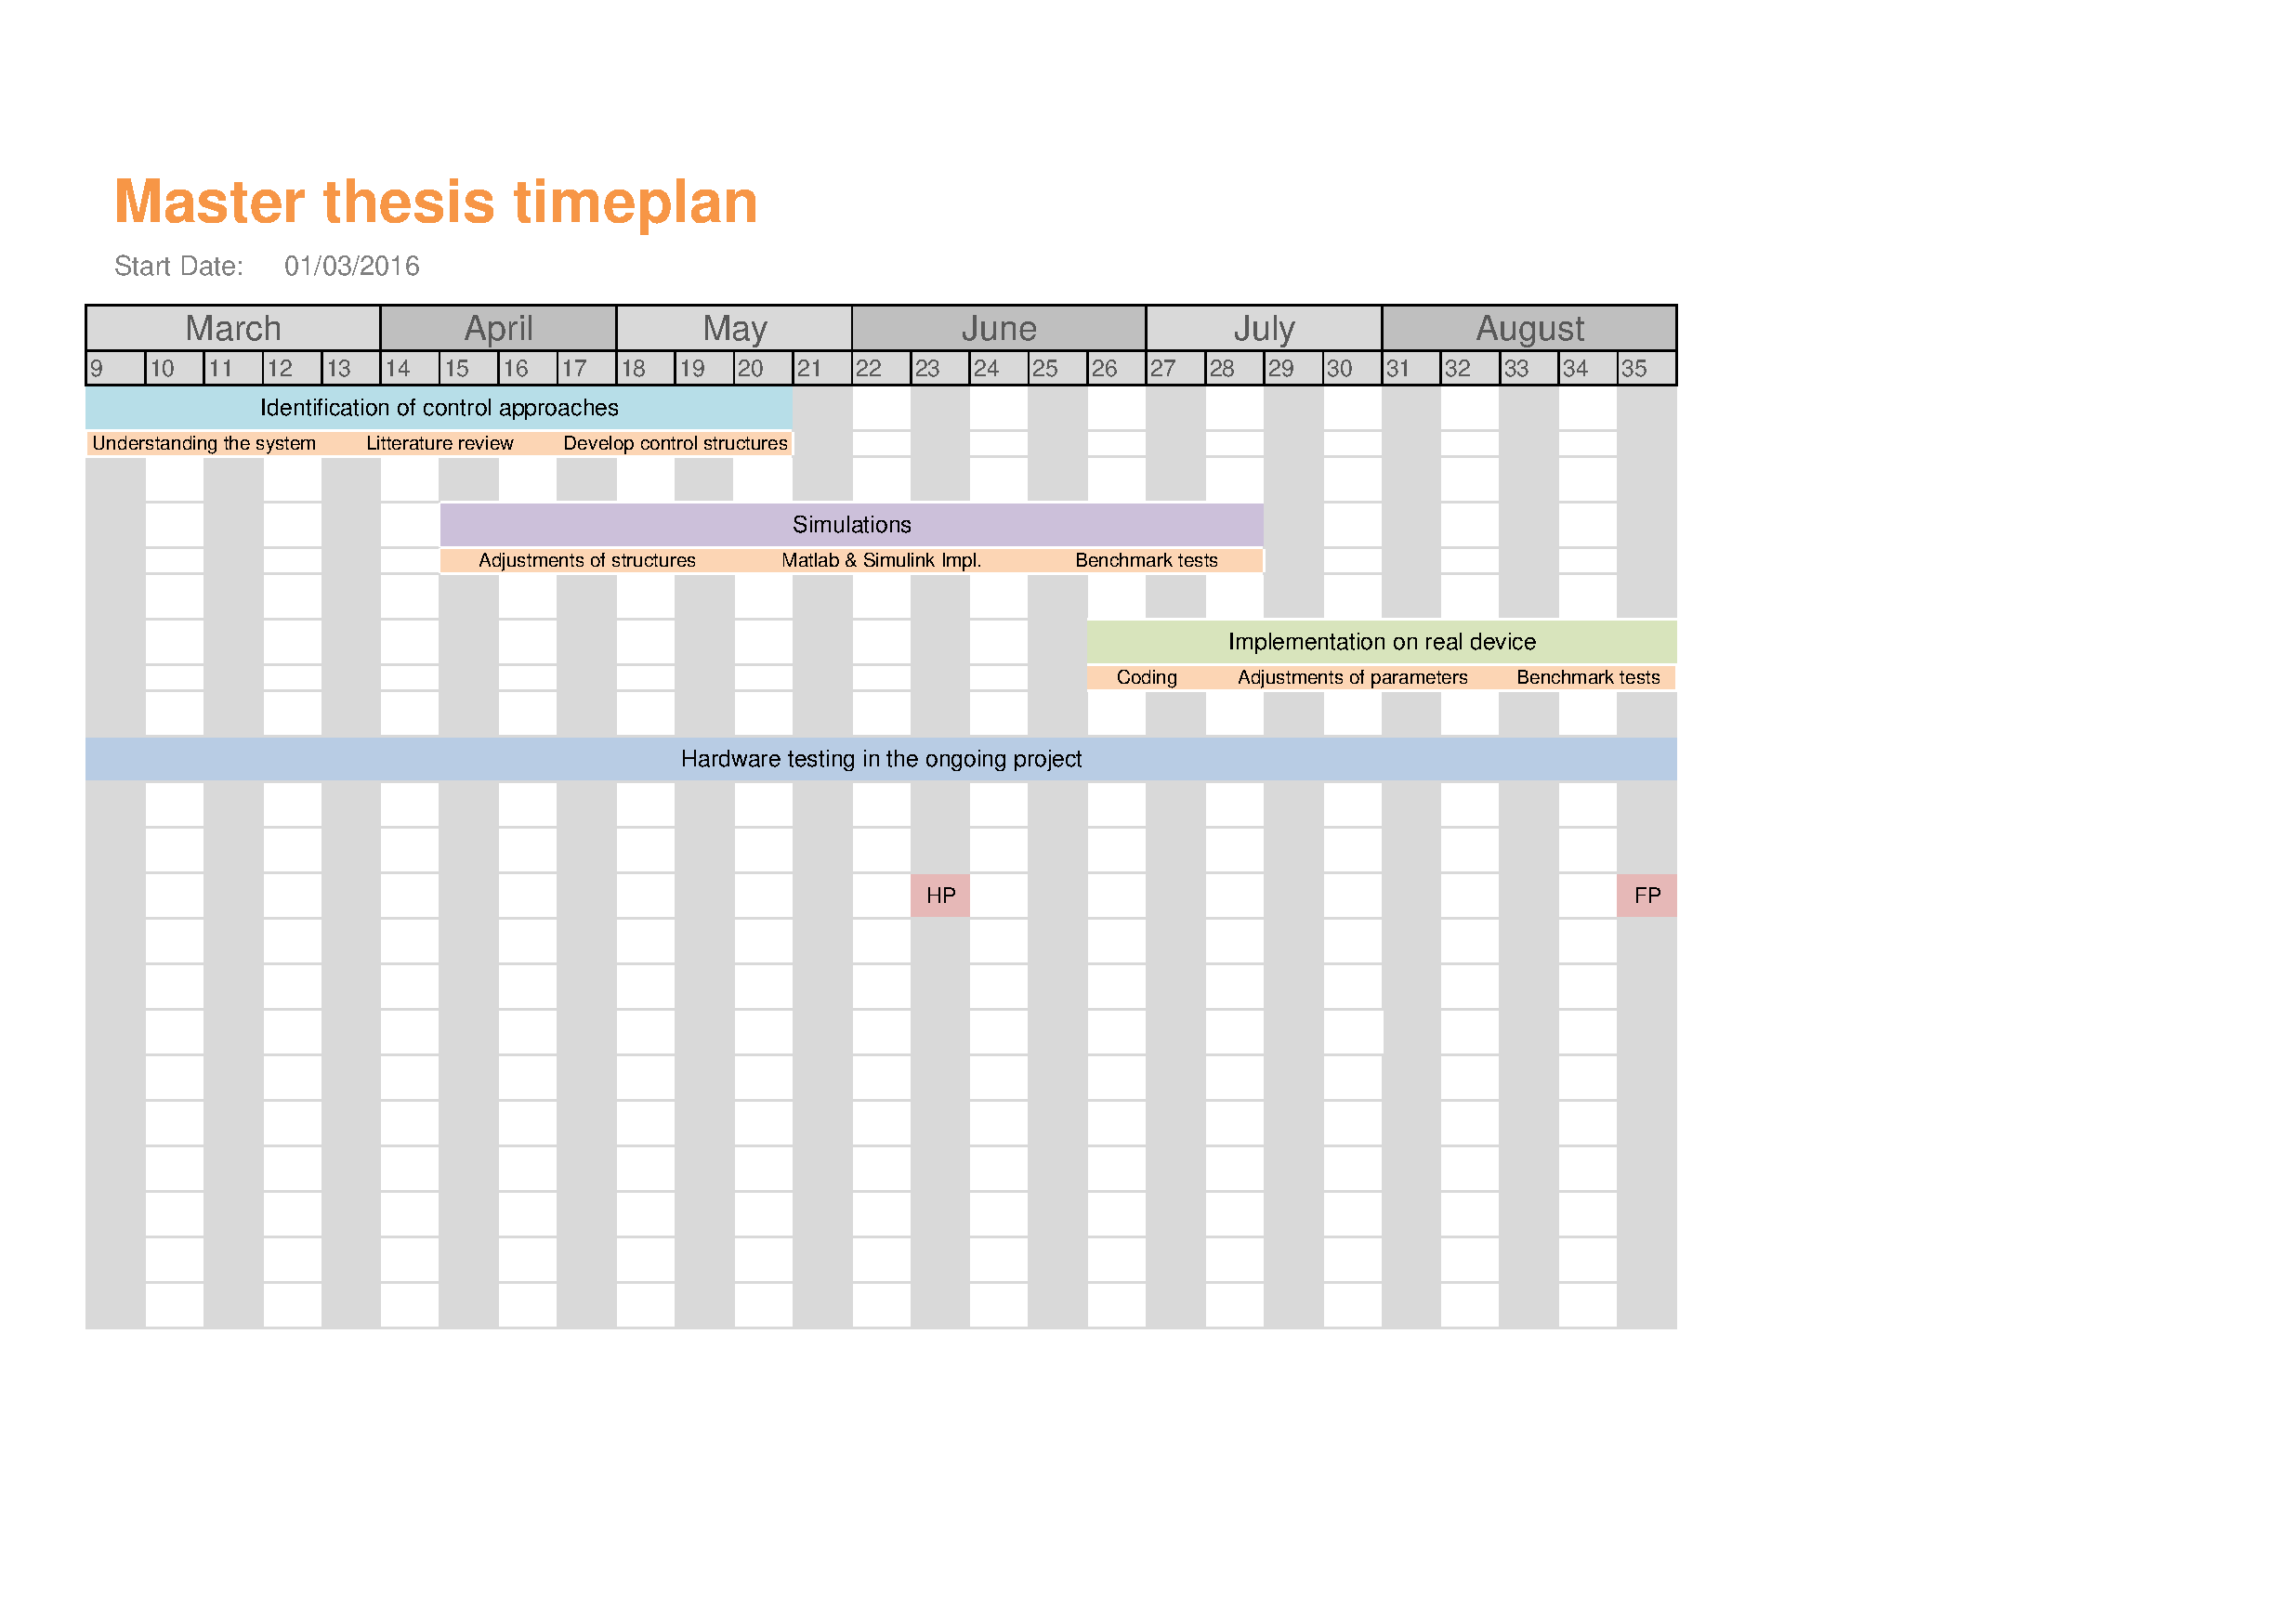
\includegraphics[trim=1cm 12cm 5cm 5.5cm, clip=true, scale=0.42]{fig/timeplan}
 \caption{\label{fig:timeplan}%
 Master Thesis timeplan}
 \end{figure}

% % !TEX root = main.tex
%preliminära resultat som kan demonstreras vid halvtidskontroll
\chapter{Result}\label{cha:result}
This section describes future results that could be expected half way through the project.

\section{Control Approaches}
Half way through the project, all control approaches that have been identified should be presented here. Furthermore, all control approaches that at the time have been simulated will be presented with a schematic structure, transfer functions or state space model, a bode plot of the closed loop system and additional plots for illustration of the trajectory tracking capability and the robustness.

\section{Benchmark tests}
Benchmark tests will be carried out on all simulated control approaches and presented here. Comparisons between the new control approaches and the existing algorithm with respect to disturbance rejection, trajectory tracking and closed loop bandwidth will be illustrated in this section with plots and tables.

% %Sätt av ett kort kapitel sist i rapporten till att avrunda och föreslå rikningar för framtida utveckling av arbetet.
% !TEX root = main.tex
\chapter{Conclusion}\label{cha:conclusion}

This thesis aims to identify, simulate and implement a suitable control approach for a piezo actuated rotational stage at \abbrCERN. The rotational stage is to be used within the UA9 project to position a bent crystal (which will steer particle beams) with a high accuracy. Several control approaches will be simulated in order to find a controller that meet the requirements. The best performing approach will be implemented and tested on the real device. 


\part*{Appendix}
\appendix
%
\chapter{definitions}\label{cha:definition}

\section{Test}

\clearemptydoublepage

\backmatter

\bibliography{IEEEfull,myrefs}

\printindex

\end{document}
